\section{A ground-truth recovery study}\label{sec:validation}

We exercise the framework in two complementary ways. First we show that the four
worked examples together exercise the object-centric constructs the construction must absorb, one
notation at a time. Then we run the construction end to end on a constructed object-centric log,
discovering two notations from the same data and checking that both recover a known ground-truth
signature. The second part is the detailed case study, and it exhibits the notation-independence of
Section~\ref{sec:general-framework} on discovered models rather than on hand-built ones.

\subsection{Coverage across the notation space}\label{subsec:coverage}

Table~\ref{tab:coverage} records the object-centric construct each notation section
stresses. Every notation is object-typed throughout, and each adds one feature the construction
absorbs uniformly. Taken together the four examples cover typing, object multiplicity,
true concurrency, silent routing, iteration, and inclusive choice, and the same
construction reduces each to its cospan signature.

\begin{table*}[t]
  \centering
  \caption{Object-centric constructs exercised by the four worked examples. Each notation is
    reduced to its cospan signature by the single construction of
    Section~\ref{sec:general-framework}.}
  \label{tab:coverage}
  \begin{tabular}{l c c c c c c l}
    \hline
    & typing & mult. & conc. & silent & loop & OR & example \\
    \hline
    OCPN   & \checkmark &            & \checkmark & \checkmark &            &            & Ex.~\ref{ex:running-pn-cospan} \\
    OCCN   & \checkmark & \checkmark & \checkmark &            &            &            & Ex.~\ref{ex:running-cnet-cospan} \\
    OCPT   & \checkmark &            & \checkmark &            & \checkmark &            & Ex.~\ref{ex:running-ptree-cospan}, \ref{ex:running-ptree-loop} \\
    OCBPMN & \checkmark &            & \checkmark &            &            & \checkmark & Ex.~\ref{ex:running-bpmn-cospan}, \ref{ex:bpmn-or} \\
    \hline
  \end{tabular}
\end{table*}

\subsection{Two discoveries, nested signatures}\label{subsec:recovery}

The case study runs the construction on a single object-centric event log and asks
how the signatures of two different discovery algorithms, applied to the same data, relate to each
other and to the process that produced the data. We fix a known ground-truth model, generate a log
from it, discover an object-centric Petri net and an object-centric causal net, extract a signature
from each, and compare the signatures and their runs.

The ground-truth model is a chest-pain serial-troponin rule-out over three object types, a
patient thread and two test channels for troponin and ECG. A round examines the patient and reads one
troponin and one ECG. The round continues only while both come back clear, and it stops at a
disposition otherwise. We define the model directly as a signature $\Sigma_{\mathrm{GT}}$ in the form of
Section~\ref{sec:general-framework}, with no model to extract it from. Its 48 generators are written
from these rules, each leg carrying one object. A round sends the patient to a next step that agrees
with both results, each result goes on to an activity that reads it, and a case leaves through one
disposition. The model is object-centric by construction and carries a loop.

We keep the ground-truth model free of key-bound object-distribution relations, the
shared-key partitions that an object-centric causal net can express but an object-centric Petri net
cannot recover. This is deliberate. On a clinically meaningful process that stays within the
constructs both notations recover, we can ask whether two independent discoveries agree, rather than
picking an example whose behaviours the two notations could never match and where a disagreement
would say nothing.

We build the object-centric event log from $\Sigma_{\mathrm{GT}}$ by a selection of its closed
runs. A start generator places one patient, one lab and one imaging object before \emph{arrive}, an
end generator takes them after \emph{depart}, and the selected runs hold at most two
re-examinations. Every linear extension of every selected run becomes one case. Each leg carries one
object, so each object type forms one chain of typed wires through a run, and a case relates one
patient, one lab and one imaging object. The log is therefore constructed rather than observed, a
point we return to below. From the log we discover an object-centric Petri net with the
standard algorithm of \citet{vanderaalstDiscoveringObjectCentricPetri2020} and an object-centric
causal net with the object-centric causal-net miner of \citet{lissObjectCentricCausalNets2025}. Each discovered model is passed through the construction of
Section~\ref{sec:general-framework} to extract its cospan signature. As diagrams the two discovered
models look quite different (Figure~\ref{fig:ed-native-models}), and their signatures below
record exactly how they differ.

\begin{figure*}[tp]
  \centering
  \begin{subfigure}[b]{0.85\linewidth}
    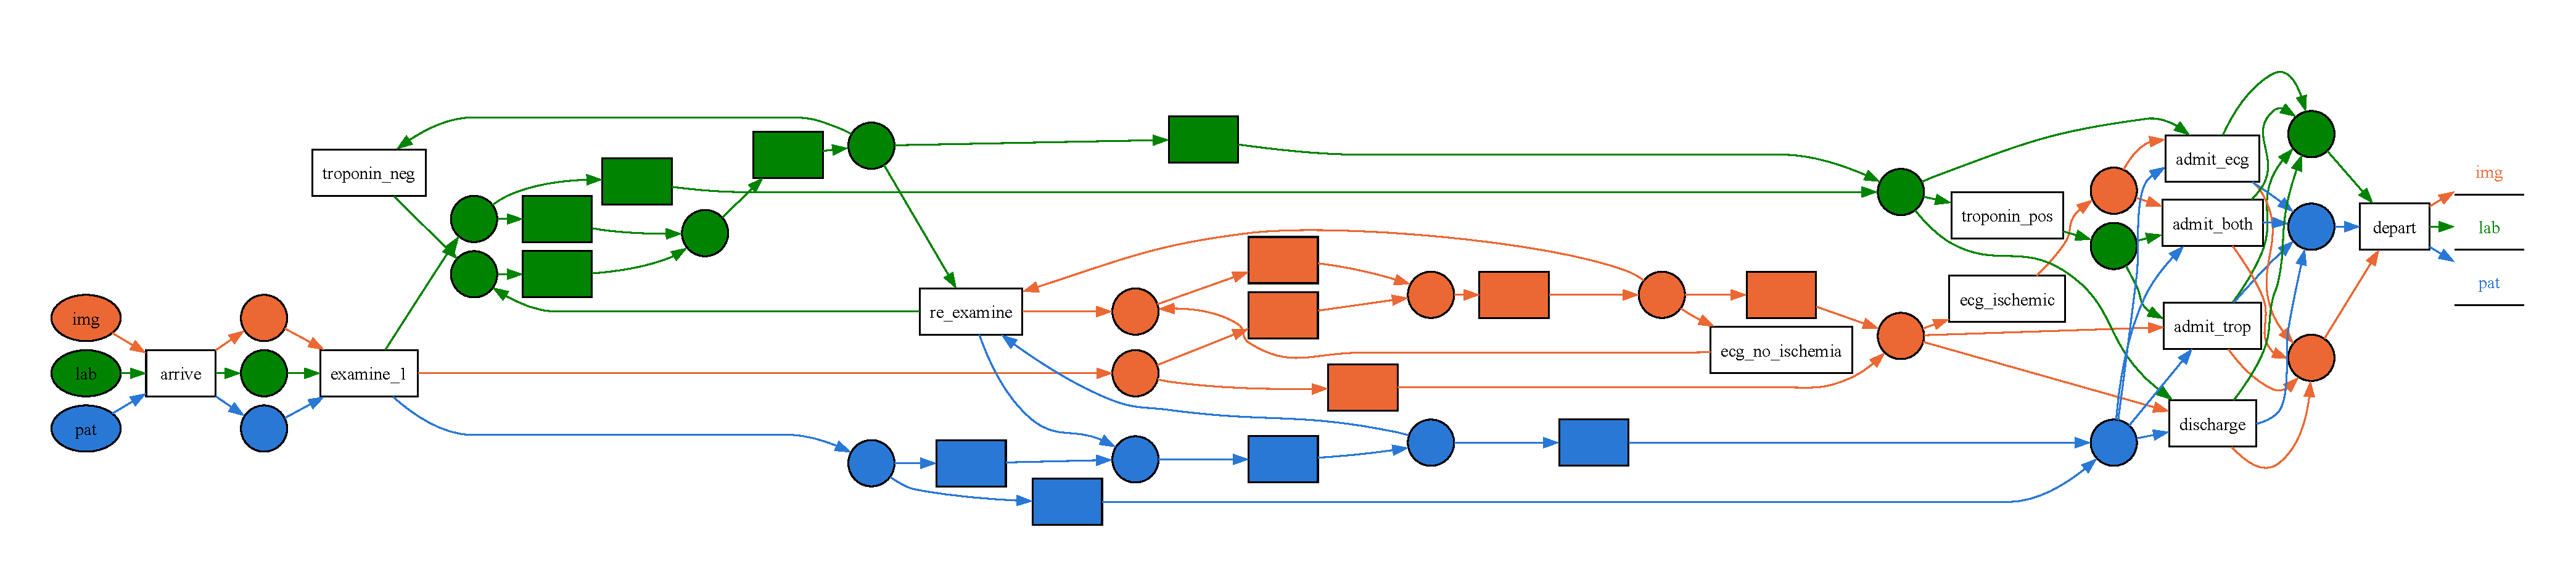
\includegraphics[width=\linewidth]{tikz/ed_chest_pain/native_ocpn.pdf}
    \caption{discovered object-centric Petri net}
  \end{subfigure}
  \\[1.5ex]
  \begin{subfigure}[b]{0.85\linewidth}
    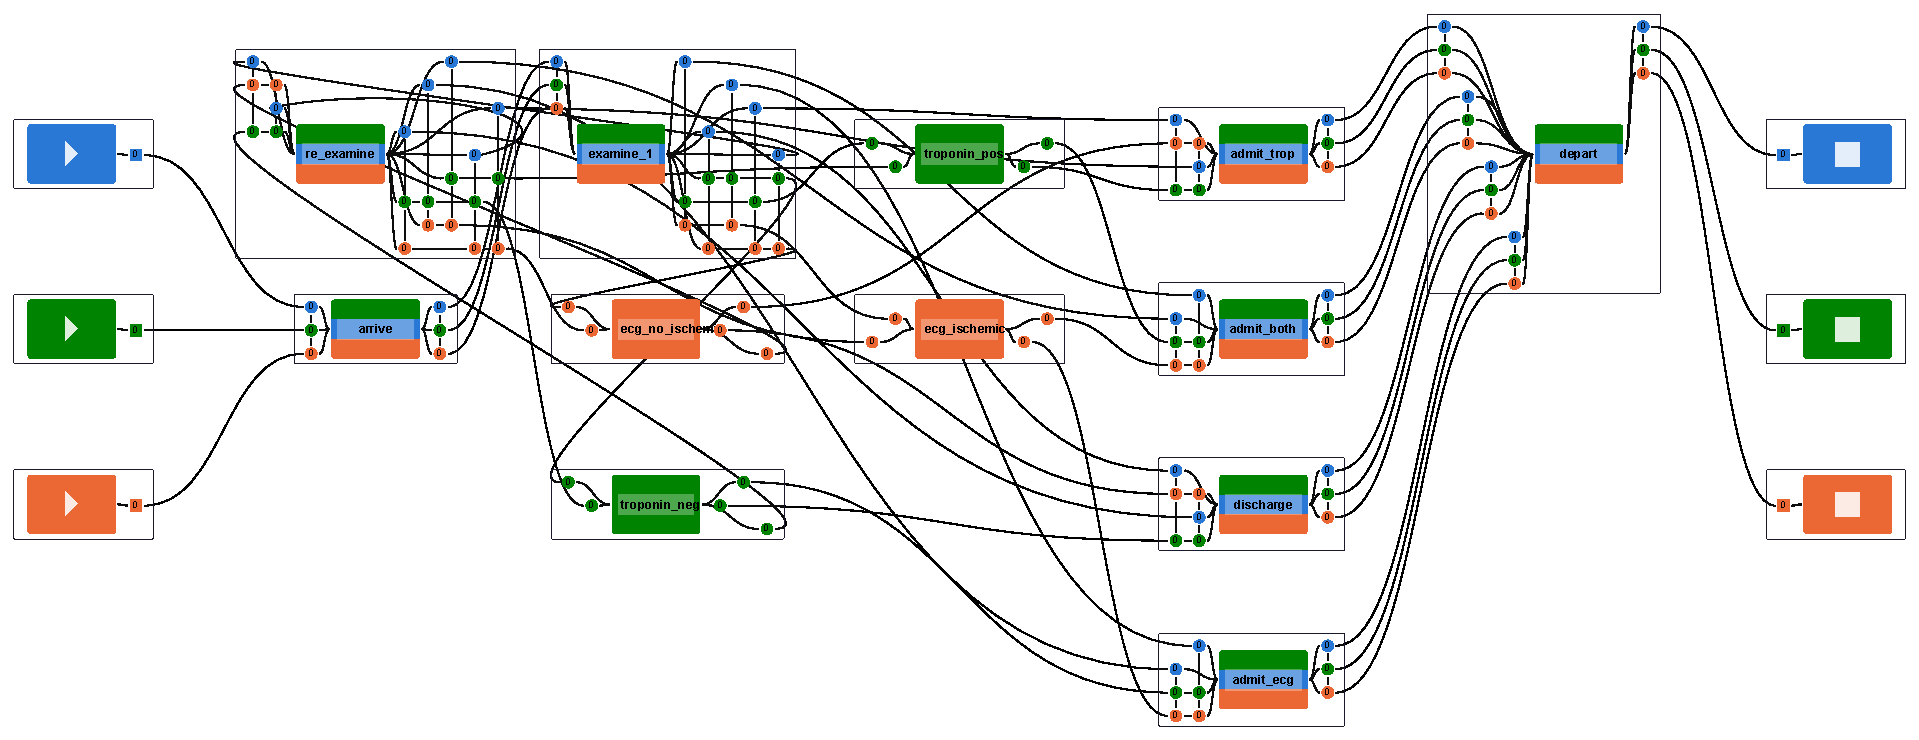
\includegraphics[width=\linewidth]{tikz/ed_chest_pain/native_occn_react.pdf}
    \caption{discovered object-centric causal net, in the reference interactive visualiser of
      \citet{lissObjectCentricCausalNets2025}}
  \end{subfigure}
  \caption{Models discovered from the same ED chest-pain log. Panel~(a) is an object-centric Petri
    net and panel~(b) an object-centric causal net, drawn in the reference interactive visualiser of
    Liss et al. The typed wires of the two extracted signatures are compared in
    Figure~\ref{fig:ed-wire-incidence}.}
  \label{fig:ed-native-models}
\end{figure*}

The extraction of Section~\ref{sec:general-framework} gives the causal net 48 generators and the
Petri net 2514. The causal-net signature is equal to $\Sigma_{\mathrm{GT}}$, generator for
generator, with the same labels, typed wires and constraint systems and the same start and end
generators. Every generator of $\Sigma_{\mathrm{GT}}$ is also equal to a generator of the Petri net,
so
\[
  \Sigma_{\mathrm{CN}}=\Sigma_{\mathrm{GT}}\subsetneq\Sigma_{\mathrm{PN}}.
\]
By Theorem~\ref{thm:canonical-presentation} the causal net has the language of the ground truth under
every selection, and by Corollary~\ref{cor:signature-inclusion} the Petri net's language contains it
under every monotone selection. The rest of this section shows
where the two differ, first on typed wires and generators and then on runs.

\begin{figure}[t]
  \centering
  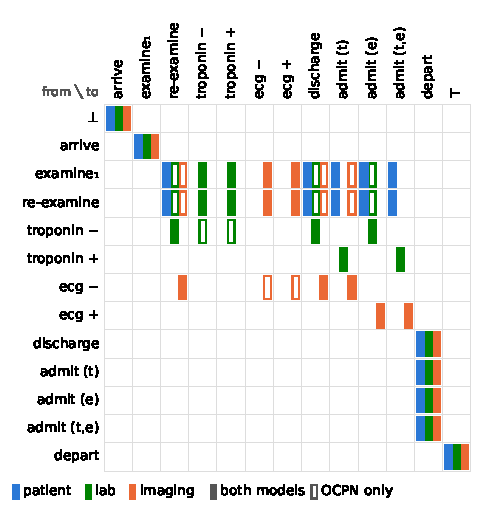
\includegraphics[width=0.9\linewidth]{tikz/ed_chest_pain/wire_incidence_spec.pdf}
  \caption{Typed wires of the two extracted signatures. A cell in row $a$ and column $b$ holds the
    typed wires $(a,w,b)$, coloured by object type. Solid cells occur in both signatures, 49 typed
    wires in all. The 16 hollow cells occur only in the object-centric Petri net, and each is a silent
    skip in one per-type net of the discovered Petri net.}
  \label{fig:ed-wire-incidence}
\end{figure}

Figure~\ref{fig:ed-wire-incidence} compares the typed wires. The causal net's 49 typed wires all
occur in the Petri net, which has 16 more. Each of the 16 is a silent skip in one of the per-type nets
the Petri-net discovery produces. The lab and imaging wires from \emph{examine} to
\emph{re-examine}, for instance, pass two silent transitions that route a test object past its test.

The wire chart is a projection of the signature and records which typed wires meet at an activity
and not which of them occur together in one generator. Every generator of either model takes one
typed wire per object type on each side, so choosing such a wire in every possible way bounds the
number of generators an activity can have. The Petri net meets
that bound at every activity, since its discovery builds one net per object type and joins them at
the activity, so the chart determines all 2514 of its generators. The causal net keeps 48 of the 153
combinations its own typed wires allow, because its bindings keep the object types of an activity
correlated. At \emph{re-examine} the chart allows 40 combinations and the causal net has 10, two input
bindings with five output bindings, since the next step of the patient must agree with both test
results. Of the Petri net's 2466 further generators, 2361 use a silent-skip wire and 105 combine
shared typed wires in ways the causal net never records.

The runs are compared under one selection. A start generator places one patient, one lab and one
imaging object before \emph{arrive}, and an end generator takes them after \emph{depart}. Both
signatures receive the same start and end generators, so the selection is monotone and the
inclusion of signatures carries over to their closed runs. The runs of both models are built from
the same pieces. A round holds some clear troponin and ECG results and ends in a re-examination,
\[
  R_{b,c}=\bigl((\mathrm{Tro}^{-})^{b}\otimes(\mathrm{ECG}^{-})^{c}\bigr)\,;\,\mathrm{Rex},
\]
where a power $f^{b}=f;\cdots;f$ is $b$ copies of $f$ composed in sequence, here $b$ clear troponin
results on the lab wire and $c$ clear ECG results on the imaging wire. A list $u=((b_1,c_1),\dots,(b_a,c_a))$ of any length $a\geq0$ gives
$R_u=R_{b_1,c_1};\cdots;R_{b_a,c_a}$, with $R_u$ the identity for the empty list. The order of the
list matters, since two rounds swapped give a different diagram.

Every closed run of either model is one of four classes, one per disposition $D$,
\[
  \mathrm{Arr}\,;\,\mathrm{Exa}_1\,;\,X\,;\,F_D\,;\,D\,;\,\mathrm{Dep},
\]
with $X$ and $F_D$ given in Table~\ref{tab:ed-run-classes}. The causal net's rounds are all clear
rounds $C_1=R_{1,1}$, so $X=C_1^{\,n}$ and a run has the single index $n$, and before its disposition
it holds exactly one result per test. These four classes are the closing diagrams of
Figure~\ref{fig:ed-decomposition} with $C_1$ inserted $n$ times. The Petri net takes any list $u$ and
any counts $b'$ and $c'$ in the final part, and Figure~\ref{fig:ed-pn-class} draws its class for
admission on the ECG.

\begin{table*}[t]
  \centering
  \caption{Run classes of the two discovered models, one per disposition $D$. Every closed run is
    $\mathrm{Arr};\mathrm{Exa}_1;X;F_D;D;\mathrm{Dep}$, with $X=C_1^{\,n}$ for the causal net and
    $X=R_u$ for the Petri net. A power is repeated sequential composition, and all indices range
    over $\mathbb{N}$.}
  \label{tab:ed-run-classes}
  \small
  \begin{tabular}{@{}l l l@{}}
    \hline
    $D$ & $F_D$, causal net & $F_D$, Petri net \\
    \hline
    Dis & $\mathrm{Tro}^{-}\otimes\mathrm{ECG}^{-}$ & $(\mathrm{Tro}^{-})^{b'}\otimes(\mathrm{ECG}^{-})^{c'}$ \\
    Adm$_{\mathrm{t}}$ & $\mathrm{Tro}^{+}\otimes\mathrm{ECG}^{-}$ & $((\mathrm{Tro}^{-})^{b'};\mathrm{Tro}^{+})\otimes(\mathrm{ECG}^{-})^{c'}$ \\
    Adm$_{\mathrm{e}}$ & $\mathrm{Tro}^{-}\otimes\mathrm{ECG}^{+}$ & $(\mathrm{Tro}^{-})^{b'}\otimes((\mathrm{ECG}^{-})^{c'};\mathrm{ECG}^{+})$ \\
    Adm$_{\mathrm{te}}$ & $\mathrm{Tro}^{+}\otimes\mathrm{ECG}^{+}$ & $((\mathrm{Tro}^{-})^{b'};\mathrm{Tro}^{+})\otimes((\mathrm{ECG}^{-})^{c'};\mathrm{ECG}^{+})$ \\
    \hline
  \end{tabular}
\end{table*}

\begin{figure*}[tp]
  \centering
  \begin{tabular}{@{}c@{\hspace{0.03\linewidth}}c@{}}
    \resizebox{0.48\linewidth}{!}{\input{tikz/ed_chest_pain/closing_1_discharge}\unskip} &
    \resizebox{0.48\linewidth}{!}{\input{tikz/ed_chest_pain/closing_2_admit_trop}\unskip} \\
    \resizebox{0.48\linewidth}{!}{\input{tikz/ed_chest_pain/closing_3_admit_ecg}\unskip} &
    \resizebox{0.48\linewidth}{!}{\begin{tikzpicture}[
    act/.style={morphismblue, font=\footnotesize, inner sep=1pt},
    patw/.style={thick, draw=typepat},
    labw/.style={thick, draw=typelab},
    imgw/.style={thick, draw=typeimg},
    seam/.style={dashed, thick, gray!70},
    seamdot/.style={circle, draw=gray!65, fill=gray!25, minimum size=3.2pt, inner sep=0pt},
    ptitle/.style={font=\small\bfseries, inner sep=2pt}]

  \useasboundingbox (-0.15,-0.55) rectangle (5.45,2.6);
  \begin{scope}[xshift=0.00cm]

  \draw[patw] (0,1.30) -- (5.25,1.30);
  \draw[labw] (0,0.65) -- (5.25,0.65);
  \draw[imgw] (0,0.00) -- (5.25,0.00);

  \node[act, minimum width=0.95cm, minimum height=1.9cm] at (0.82,0.65) {Exa$_1$};
  \node[act, minimum width=0.95cm, minimum height=0.48cm] at (2.62,0.65) {Tro$+$};
  \node[act, minimum width=0.95cm, minimum height=0.48cm] at (2.62,0.00) {ECG$+$};
  \node[act, minimum width=0.95cm, minimum height=1.9cm] at (4.42,0.65) {Adm$_{\mathrm{te}}$};

  \draw[seam] (1.72,-0.40) -- (1.72,1.72);
  \foreach \y in {1.30,0.65,0.00} \node[seamdot] at (1.72,\y) {};
  \node[font=\small, gray!80, anchor=south, inner sep=1pt] at (1.72,1.72) {$C_1^{\,n}$};

  \node[ptitle] at (2.62,2.35) {Closing 4 (both $+$)};
  \end{scope}
\end{tikzpicture}
\unskip} \\
    \resizebox{0.48\linewidth}{!}{\begin{tikzpicture}[
    act/.style={morphismblue, font=\footnotesize, inner sep=1pt},
    patw/.style={thick, draw=typepat},
    labw/.style={thick, draw=typelab},
    imgw/.style={thick, draw=typeimg},
    seam/.style={dashed, thick, gray!70},
    seamdot/.style={circle, draw=gray!65, fill=gray!25, minimum size=3.2pt, inner sep=0pt},
    ptitle/.style={font=\small\bfseries, inner sep=2pt}]

  \useasboundingbox (-0.15,-0.55) rectangle (5.45,2.6);
  \begin{scope}[xshift=0.90cm]

  \draw[patw] (0,1.30) -- (3.45,1.30);
  \draw[labw] (0,0.65) -- (3.45,0.65);
  \draw[imgw] (0,0.00) -- (3.45,0.00);

  \node[act, minimum width=0.95cm, minimum height=0.48cm] at (0.82,0.65) {Tro$-$};
  \node[act, minimum width=0.95cm, minimum height=0.48cm] at (0.82,0.00) {ECG$-$};
  \node[act, minimum width=0.95cm, minimum height=1.9cm] at (2.62,0.65) {Rex};

  \draw[seam] (0.17,-0.40) -- (0.17,1.72);
  \foreach \y in {1.30,0.65,0.00} \node[seamdot] at (0.17,\y) {};
  \draw[seam] (3.28,-0.40) -- (3.28,1.72);
  \foreach \y in {1.30,0.65,0.00} \node[seamdot] at (3.28,\y) {};

  \node[ptitle] at (1.73,2.35) {$C_1$ (both-clear round)};
  \end{scope}
\end{tikzpicture}
\unskip} &
    \resizebox{0.48\linewidth}{!}{\begin{tikzpicture}[
    act/.style={morphismblue, font=\footnotesize, inner sep=1pt},
    patw/.style={thick, draw=typepat},
    labw/.style={thick, draw=typelab},
    imgw/.style={thick, draw=typeimg},
    seam/.style={dashed, thick, gray!70},
    seamdot/.style={circle, draw=gray!65, fill=gray!25, minimum size=3.2pt, inner sep=0pt},
    ptitle/.style={font=\small\bfseries, inner sep=2pt}]
  \useasboundingbox (-0.15,-0.55) rectangle (5.45,2.6);

  \node[anchor=north west, font=\footnotesize, inner sep=0pt] at (0.20,2.45) {%
    \renewcommand{\arraystretch}{0.95}%
    \begin{tabular}{@{}l@{\quad}l@{}}
      Exa$_1$ & first examination\\
      Rex & re-examination\\
      Tro$\pm$ & troponin, $+$ or $-$\\
      ECG$\pm$ & ECG, $+$ or $-$\\
      Dis & discharge\\
      Adm$_{\mathrm{t}}$ & admit on troponin\\
      Adm$_{\mathrm{e}}$ & admit on ECG\\
      Adm$_{\mathrm{te}}$ & admit on both
    \end{tabular}};

  \draw[patw] (4.20,1.60) -- (4.65,1.60) node[anchor=west, font=\footnotesize, inner sep=2pt] {pat};
  \draw[labw] (4.20,1.10) -- (4.65,1.10) node[anchor=west, font=\footnotesize, inner sep=2pt] {lab};
  \draw[imgw] (4.20,0.60) -- (4.65,0.60) node[anchor=west, font=\footnotesize, inner sep=2pt] {img};
\end{tikzpicture}
\unskip} \\
  \end{tabular}
  \caption{The four run classes of the causal net, drawn with one horizontal channel per object
    type and without the \emph{arrive} and \emph{depart} boxes. Each closing diagram is one
    disposition, and the clear round $C_1=R_{1,1}$ is inserted $n$ times at the dashed seam. The
    dashed seams at both ends of $C_1$ mark that same interface. Box labels are abbreviated, with the
    key beside $C_1$.}
  \label{fig:ed-decomposition}
\end{figure*}

\begin{figure*}[tp]
  \centering
  \resizebox{0.9\linewidth}{!}{\begin{tikzpicture}[
    act/.style={morphismblue, font=\footnotesize, inner sep=1pt},
    patw/.style={thick, draw=typepat},
    labw/.style={thick, draw=typelab},
    imgw/.style={thick, draw=typeimg},
    pw/.style={font=\scriptsize, inner sep=0.5pt, anchor=south west},
    round/.style={dashed, thick, gray!70, rounded corners=3pt}]

  \draw[patw] (0.55,1.30) -- (11.25,1.30);
  \draw[labw] (0.55,0.65) -- (11.25,0.65);
  \draw[imgw] (0.55,0.00) -- (11.25,0.00);

  \node[act, minimum width=0.85cm, minimum height=1.9cm] at (0.55,0.65) {Arr};
  \node[act, minimum width=0.85cm, minimum height=1.9cm] at (1.90,0.65) {Exa$_1$};

  \draw[round] (2.75,-0.45) rectangle (5.75,1.75);
  \node[act, minimum width=0.85cm, minimum height=0.48cm] (t1) at (3.55,0.65) {Tro$-$};
  \node[pw] at (t1.north east) {$b_i$};
  \node[act, minimum width=0.85cm, minimum height=0.48cm] (e1) at (3.55,0.00) {ECG$-$};
  \node[pw] at (e1.north east) {$c_i$};
  \node[act, minimum width=0.85cm, minimum height=1.9cm] at (5.05,0.65) {Rex};
  \node[font=\footnotesize, gray!80, anchor=south] at (4.25,1.75) {$R_{b_i,c_i}$};
  \node[font=\footnotesize, gray!80, anchor=west] at (5.75,1.55) {$\times\, a$};
  \draw[decorate, decoration={brace, amplitude=4pt, mirror}, gray!80, thick] (2.75,-0.55) -- (5.75,-0.55)
    node[midway, below=4pt, font=\footnotesize] {$R_u$};

  \node[act, minimum width=0.85cm, minimum height=0.48cm] (t2) at (6.65,0.65) {Tro$-$};
  \node[pw] at (t2.north east) {$b'$};
  \node[act, minimum width=0.85cm, minimum height=0.48cm] (e2) at (6.65,0.00) {ECG$-$};
  \node[pw] at (e2.north east) {$c'$};
  \node[act, minimum width=0.85cm, minimum height=0.48cm] at (8.05,0.00) {ECG$+$};

  \node[act, minimum width=0.85cm, minimum height=1.9cm] at (9.45,0.65) {Adm$_{\mathrm{e}}$};
  \node[act, minimum width=0.85cm, minimum height=1.9cm] at (10.85,0.65) {Dep};

  \node[font=\scriptsize, anchor=east] at (0.05,1.30) {patient};
  \node[font=\scriptsize, anchor=east] at (0.05,0.65) {lab};
  \node[font=\scriptsize, anchor=east] at (0.05,0.00) {imaging};
\end{tikzpicture}
\unskip}
  \caption{The Petri net's run class for admission on the ECG. The dashed frame is one round
    $R_{b_i,c_i}$, and the frames for $i=1,\dots,a$ compose in order to $R_u$. A number beside a box
    counts its copies composed in sequence on that wire. The causal net's class for the same
    disposition sets $u=((1,1),\dots,(1,1))$, $b'=1$ and $c'=0$.}
  \label{fig:ed-pn-class}
\end{figure*}

A round of the Petri net may hold any number
of clear results on each test, including none, and the final part may repeat a clear result before
an abnormal one or hold no result for a test at all. Each of these uses a silent-skip wire of
Figure~\ref{fig:ed-wire-incidence}. A round without tests joins \emph{examine} or \emph{re-examine} to
\emph{re-examine} on the lab and imaging wires, a repeated result joins a clear test result to itself
or to the abnormal result of the same test, and a
disposition without a test joins \emph{examine} or \emph{re-examine} to the disposition. The two
abnormal results of an admission on both tests lie on different wires and are concurrent in one
diagram, so the two orders in which they can be logged are two linear extensions of one run and not
two classes. With every index at zero both models have four base runs. The causal net's are its four
closing diagrams. Three of the Petri net's omit a clear result the causal net requires, and only
admission on both tests keeps both.

The classes are exact. Enumerating every closed run of up to twelve occurrences, each run of the
Petri net matches one index tuple of one class, and each tuple in that bound is a run, 4180, 1596,
1596 and 609 runs for the four dispositions. The causal net's twelve runs are its classes with
$n\leq2$. The minimal automata of the two languages, with 13 and 8 states, decide the inclusion
without a length bound. The causal net's language is strictly included in the Petri net's, and the
shortest word only the Petri net admits is \emph{arrive examine discharge depart}. The causal net
therefore recovers the ground-truth signature exactly, and the Petri net's signature and language
strictly contain it.

\subsection{Applicability and limitations}\label{subsec:threats}

The extraction and comparison are implemented. A discovery output in a standard
interchange format is read into a signature, and the certificate of
Section~\ref{sec:conversion-framework} decides structural equivalence by set-equality of the two
signatures, which is convention-free and strictly finer than trace equivalence by
Lemma~\ref{lem:equiv-strictness}. Set-inclusion of signatures decides the inclusion used here.

The statement this supports runs in one direction. Equal signatures give equal trace languages,
and included signatures give included trace languages under a monotone selection. Models with
different signatures are structurally different, and whether they nonetheless agree on their trace
languages is a separate question, which the automata settle here. An inclusion of signatures, as
found here, is therefore a stronger statement than an inclusion of trace languages would be.

\paragraph{Contents of the log.}
The log is a complete enumeration and not a sample. It holds 576 events over 168 objects under
twelve event labels, one case for every linear extension of every closed run of
$\Sigma_{\mathrm{GT}}$ with at most two re-examinations. The run-space is a disposition with
$n$ copies of one clear round, the $C_1$ of Figure~\ref{fig:ed-decomposition}, inserted after the
first examination, so a single
integer $n$ characterises every unrolling and nested loops would need a set of numbers. The depth realised in the log is a free parameter of the enumeration rather than a
property of the model, and the recovery does not depend on it, because the run classes of
Table~\ref{tab:ed-run-classes} hold for every $n$. Fixing $n$ from data is an
estimation question outside the scope of this paper. The log has to be complete, because a
recovery measurement asks whether discovery returns the model that produced the log, and that
question only makes sense when the log realises that model in full. The result should be read as
establishing that the extraction is well defined and non-vacuous on discovery output, and not as
a measurement of miner robustness under noise or incompleteness. The log records the start and
end of each case as the activities \emph{arrive} and \emph{depart}, which both signatures contain.
The start and end generators of the run comparison are separate from them, belong to
$\Sigma_\gamma$ (Section~\ref{subsec:analysis}) and are stated as its assumption.

\paragraph{Reasons for a constructed log.}
The study measures recovery, which compares each discovered signature against the signature of
the model that produced the log. A ground-truth model is therefore a precondition of the
measurement rather than a property of the data that one could go looking for. No log observed in
a running information system supplies one, because the only candidate target available for such a
log is itself the output of a discovery algorithm, and scoring a discovery against a discovery
measures agreement between two miners instead of recovery of a known model. This bounds what any
public data could contribute and is not a gap in our search.

The simulated public logs do not close the gap either. The object-centric order-management log
of the OCEL 2.0 collection is generated from a coloured Petri net, and a coloured Petri net types
its tokens by colour set rather than by object type. OCEL 2.0 and coloured Petri nets are not
intrinsically coupled, and we draw this observation only for the order-management log we examined.
Reading such a model as an object-centric one fixes a
correspondence between colour sets and object types that the published artefact leaves open, so
the object structure would be ours and not the dataset's. In any case the object-centric Petri nets published
alongside these logs are obtained from the logs by discovery, and are therefore targets of the
same kind as the models under comparison.

Everything the construction does not decide is left to the two miners. Both are independently authored
third-party implementations, neither was written with cospan signatures in mind, and each targets
a different notation. The causal net's recovery of the ground-truth signature, and the inclusion of
that signature in the Petri net's, are therefore not artefacts of how the log was generated. A construction reading the generator
rather than the miners' output would agree with itself.

The absence of a ground truth in observed data is also why comparing signatures by equality and
inclusion is worth having. Where no reference model exists, two models can still be compared against each
other, and that comparison is the subject of Section~\ref{sec:conversion-framework}.

Three limitations bound these claims. The log is noise-free and enumerates the behaviour of the
ground-truth model completely, so nothing here measures what the extraction does under incomplete
traces, mislabelled activities, or missing object relations. The four worked examples are
deliberately minimal. The reverse maps of Section~\ref{sec:conversion-framework} are
one-directional. The implementation is released as the \texttt{proc-posets} package alongside the
paper.
